\chapter{Permutations, Cosets, and Direct Products}

\section{Groups of Permutations}

\begin{definition}[Permutation of a set]
    A \emph{permutation of a set} $A$ is a function $\phi\colon A \to A$ that is both one to one and onto.
\end{definition}
\begin{remark}[Permutation Multiplication]
    Function composition $\circ$ is a binary operation on the collection of all permutations of a set $A$. We call this operation \emph{permutation multiplication}.
\end{remark}
\begin{remark}
    Let $\sigma, \tau$ be permutations of a set $A$ so $\sigma, \tau$ are both one-to-one function mapping $A$ onto $A$. then, $\sigma\circ\tau$, or simply $\sigma\tau$ is a permutation as long as it is one-to-one.

    For any $a_1,a_2 \in A$, if $(\sigma\tau)(a_1)=(\sigma\tau)(a_2)$ gives $(\sigma(\tau(a_1)))=(\sigma()\tau(a_1))$. Because $\sigma$ is injective, $\tau(a_1)=\tau(a_2)$. Because $\tau$ is injective, $a_1=a_2$ so $\sigma\tau$ is injective.

    For any $a \in A$, there exists some $b in A$ so $\sigma(b) = a$ because $\sigma$ is onto $A$. Because $\tau$ is onto $A$, there exists some $c \in A$ so $\tau(c) = b$. Thus, $a = (\sigma\tau)(c)$ so $\sigma\tau$ is onto $A$.
\end{remark}
\begin{example}
    Given a set $A = \{1,2,3,4,5\}$, we can write a permutation $\sigma$ as 
    \[\sigma =
    \begin{pmatrix}
        1 & 2 & 3 & 4 & 5 \\
        4 & 2 & 5 & 3 & 1
    \end{pmatrix}.\] so $\sigma(1) = 4$, etc.
\end{example}
\begin{theorem}
    Let $A$ be a nonempty set, and $S_A$ be the collection of all permutations of $A$. Then, $S_A$ is a group under permutation multiplication.
\end{theorem}
\begin{proof}
    Because the composition of two permutations of $A$ results in a permutation, we have closure under $\circ$. For any functions $f,g,h$, $((f\circ g)\circ h)(x) = (f(g))\circ(h)(x) = f(g(h))(x) = f(g\circ h)(x)$ so $\mathscr{G}_1$ is easily satisfied. The permutation $\imath$ defined as $\imath(a)=a$ for all $a \in A$ is the identity ($\mathscr{G}_2$). Last, for any permutation $\sigma$, $\sigma^{-1}$ reverse the direction of the mapping $\sigma$ such that $\sigma^{-1}(a)$ is the element $a'$ of $A$ so $\sigma(a')=a$. This exists because $\sigma$ is bijective. For any $a \in A$, $\imath(a) = a = \sigma(a') = \sigma(\sigma^{-1}(a')) = (\sigma\sigma^{-1})(a)$ and $\imath(a') = a' = \sigma^{-1}(a) = \sigma^{-1}(\sigma(a')) = (\sigma^{-1}\sigma)(a')$ satisfying $\mathscr{G}_3.$
\end{proof}
\begin{remark}
    To define an isomorphism $\phi\colon S_A \to S_B$, we let $f \colon A \to B$ have one-to-one function mapping $A$ onto $B$ so $A$ and $B$ have the same cardinality so for $\sigma \in S_A$, let $\phi(\sigma) = \bar{\sigma}\in S_B$ so that for all $a \in A$, $\bar{\sigma}(f(a)) = f(\sigma(a)).$ 
\end{remark}
\begin{definition}[Symmetric Group on $n$ Letters]
    Let $A$ be the finite set $\{1,2,\dots,n\}$. The group of all permutations of $A$ is the \emph{symmetric group on $n$ letters} $S_n$. Note that $S_n$ has $n!$ elements.
\end{definition}
\begin{remark}
    $S_3$ is also the 3rd dihedral group $D_3$ of \emph{symmetries of an equilateral triangle} where $\rho_i$ is rotations and $\mu_i$ is mirror images in bisectors of angles such that $D_3$ is made up of:
    \[
    \begin{Bmatrix}
        \rho_0 = \begin{pmatrix} 1 & 2 & 3 \\ 1 & 2 & 3 \end{pmatrix}, &
        \mu_0 = \begin{pmatrix} 1 & 2 & 3 \\ 1 & 3 & 2 \end{pmatrix}, \\
        \rho_1 = \begin{pmatrix} 1 & 2 & 3 \\ 2 & 3 & 1 \end{pmatrix}, &
        \mu_1 = \begin{pmatrix} 1 & 2 & 3 \\ 3 & 2 & 1 \end{pmatrix}, \\
        \rho_2 = \begin{pmatrix} 1 & 2 & 3 \\ 3 & 1 & 2 \end{pmatrix}, &
        \mu_2 = \begin{pmatrix} 1 & 2 & 3 \\ 2 & 1 & 3 \end{pmatrix}.        
    \end{Bmatrix}
    \]
\end{remark}
\begin{definition}[$n$th Dihedral Group $D_n$]
    The \emph{$n$th dihedral group $D_n$} is the group of symmetries of the regular $n$-gon.
\end{definition}
\begin{example}[Octic Group $D_4$]
    Given a square: 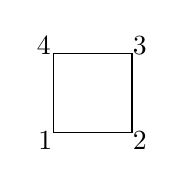
\begin{tikzpicture}
        \draw (0cm,0cm) rectangle (1cm, 1cm);
        \foreach \x/\y/\n in {-.1/-.1/1, 1.1/-.1/2, 1.1/1.1/3, -.12/1.1/4}{\node at (\x cm, \y cm) {\n};}\end{tikzpicture}
    , $D_4$ is the set of:
    \[
        \begin{Bmatrix}
            \rho_0 = \begin{pmatrix} 1 & 2 & 3 & 4\\ 1 & 2 & 3 & 4 \end{pmatrix}, &
            \mu_0 = \begin{pmatrix} 1 & 2 & 3 & 4 \\ 2 & 1 & 4 & 3 \end{pmatrix}, \\
            \rho_1 = \begin{pmatrix} 1 & 2 & 3 & 4\\ 2 & 3 & 4 & 1 \end{pmatrix}, &
            \mu_1 = \begin{pmatrix} 1 & 2 & 3 & 4 \\ 4 & 3 & 2 & 1 \end{pmatrix}, \\
            \rho_2 = \begin{pmatrix} 1 & 2 & 3 & 4\\ 3 & 4 & 1 & 2 \end{pmatrix}, &
            \delta_0 = \begin{pmatrix} 1 & 2 & 3 & 4 \\ 3 & 2 & 1 & 4 \end{pmatrix}, \\
            \rho_3 = \begin{pmatrix} 1 & 2 & 3 & 4\\ 4 & 1 & 2 & 3 \end{pmatrix}, &
            \delta_1 = \begin{pmatrix} 1 & 2 & 3 & 4 \\ 1 & 4 & 3 & 2 \end{pmatrix}.
        \end{Bmatrix}
        \]
    where $\rho_i, \mu_i, \delta_i$ represent rotations, mirror images in perpendicular bisectors of sides, and diagonal flips respectively.
\end{example}
\begin{definition}[Image of $H$ under $f$]
    Let $f\colon A\to B$ be a function and $H$ be a subset of $A$. The \emph{image of $H$ under $f$} is the set $\{f(h) \mid h \in H\}$ and is denoted $f[H].$
\end{definition}
\begin{lemma}
    Let $G, G'$ be groups and $\phi\colon G\to G'$ be a one-to-one function such that for all $x,y \in G$, $\phi(xy) = \phi(x)\phi(y).$ Thus $\phi[G]$ is a subgroup of $G'$ and $\phi$ provides an isomorphism of $G$ with $\phi[G]$.
\end{lemma}
\begin{proof}
    We simply prove the subgroup requirements. For any $x', y' \in \phi[G]$, there exist $x,y \in G$ so $\phi(x)=x'$ and $\phi(y)=y'$. By hypothesis, $\phi(xy) = \phi(x)\phi(y)$ so $x'y' \in \phi[G]$ so $\phi[G]$ is closed under the operation of $G'$. Next, say $e'$ is the identity of $G'$. Then, $e'\phi(e) = \phi(e) = \phi(ee) = \phi(e)\phi(e)$. Cancellation in $G'$ shows $e'=\phi(e)$ so $e' \in \phi[G]$. Last, for any $x' \in \phi[G]$, $e'=\phi(e)=\phi(xx^{-1})=\phi(x)\phi(x^{-1})=x'\phi(x^{-1})$ implying $x'^{-1} = \phi(x^{-1}) \in \phi[G]$. Thus $\phi[G]$ is a subgroup of $G'$. We already showed $\phi$ is onto and therefore an isomorphism of $G$ with $\phi[G]$.
\end{proof}
\begin{theorem}[Cayley's Theorem]
    Every group is isomorphic to a group of permutations.
\end{theorem}
\begin{proof}
    Let $G$ be a group. We want to show $G$ is isomorphic to a subgroup of $S_G$. By the previous lemma, we need only define a universal one-to-one function $\phi\colon G\to S_G$ with the homomorphism property. For any $x,g \in G$, let's define left multiplication by x via $\lambda_x\colon G\to G$ as $\lambda_x(g)=xg$. For all $c \in G$, $\lambda_x(x^-1c)=x(x^-1c)=c$ so clearly $\lambda_x$ maps $G$ onto $G$. Also, for any $a,b \in G$, $\lambda_x(a)=\lambda_x(b) \implies xa=xb \implies a=b$ through left cancellation. Thus, $\lambda_x$ is one-to-one, onto, and a permutation of $G$. Now, we define $\phi\colon G\to S_G$ as $\phi(x)=\lambda_x$ for all $x\in G$.

    To satisfy our lemma, we now only show $\phi$ is one-to-one and has the homomorphism property. Let $e$ be the identity on $G$ so that $\phi(x)=\phi(y)$ implies $\lambda_x=\lambda_y$ so $\lambda_x(e)=\lambda_y(e)\implies xe=ye \implies x=y$. Last, for any $x,y,g\in G$, $\lambda_{xy}(g) = (xy)g = x(yg) = \lambda_x(\lambda_y(g)) = \lambda_x\lambda_y(g)$ so $\phi(xy)=\phi(x)\phi(y)$ satisfying the homomorphism property.
\end{proof}
\begin{definition}[Left/Right Regular Representation]
    The map $\phi\colon G \to S_G$ defined as above is the \emph{left regular represention} of $G$ and the map $\mu\colon G \to S_G$ defined by $\mu(x)=\rho_{x^{-1}}$ where $\rho_x(g)=gx$ for all $x,g\in G$ is the \emph{right regular representation} of $G$.
\end{definition}

\section{Orbits, Cycles, and the Alternating Groups}

\begin{definition}[Orbit of $a$ under $\sigma \in S_A$]
    Let $A$ be a set and $\sigma \in S_A$. For a fixed $a \in A$, the set $\mathcal{O}_{a.\sigma}=\{\sigma^n(a)\mid n\in\Z\}$ is the \emph{orbit of $a$ under $\sigma$.}
\end{definition}
\begin{remark}
    Let $\sigma$ be a permutation of a set $A$. The equivalence classes in $A$ are determined by the following equivalence class:
    \begin{center}
        For $a,b \in A$, let $a\sim b$ if and only if $b = \sigma^n(a)$ for some $n \in \Z$.
    \end{center}
    These are called the \emph{orbits of $\sigma$}.
\end{remark}
\begin{explanation}
    $\sim$ is an equivalence relation because it is:
    \begin{enumerate}
        \item \textbf{reflexive:} $a\sim a$ clearly because $a=\imath(a)=\sigma^0(a)$.
        \item \textbf{symmetric:} If $a \sim b$, then $b = \sigma^n(a)$ for some $n \in \Z$ so $a = \sigma^{-n}(b)$ and $-n \in \Z$ so $b\sim a$.
        \item \textbf{transitive:} If $a \sim b, b \sim c$, then $b = \sigma^n(a)$ and $c = \sigma^m(b)$ for some $n,m \in \Z$. This implies $c = \sigma^m(\sigma^n(a)) = \sigma^{n+m}(a)$ so $a \sim c$.
    \end{enumerate}
\end{explanation}
\begin{example}
    The orbits of $\imath$ are the singleton subsets of $A$.
\end{example}
\begin{example}
    Given the permutation $\sigma$ of a finite set $A$ defined as:
    \[\sigma = \begin{pmatrix}
        1 & 2 & 3 & 4 & 5 & 6 & 7 & 8 \\ 3 & 8 & 6 & 7 & 4 & 1 & 5 & 2
    \end{pmatrix},\]
    the complete list of orbits of $\sigma$ are $$\{1,3,6\}, \; \{2,8\}, \; \text{and }\{4,5,7\},$$ which we can map in the following way:
    \begin{center}
        \begin{tikzpicture}
            \node [circle, draw, minimum size = 2cm, postaction={decorate}, decoration={markings, mark=between positions .083 and 1.000 step 0.333 with {\arrow{>}}}] (1) at (0,0) {};
            \node [circle, draw, minimum size = 2cm, postaction={decorate}, decoration={markings, mark=between positions .500 and 1.000 step 0.500 with {\arrow{>}}}] (2) at (3cm, 0) {};
            \node [circle, draw, minimum size = 2cm, postaction={decorate}, decoration={markings, mark=between positions .083 and 1.000 step 0.333 with {\arrow{>}}}] (3) at (6cm, 0) {};

            \foreach \n/\circ/\rad\direc in {1/1/-.083/right, 3/1/.250/above, 6/1/.583/left, 2/2/.250/above, 8/2/.750/below, 4/3/.250/above, 7/3/.583/left, 5/3/.916/right}
            {
                \node[draw, thick, fill, inner sep = .3mm, circle, label = \direc:\n] at (\circ.\rad*360) {};
            }
        \end{tikzpicture}
    \end{center}
\end{example}
\begin{definition}
    A permutation $\sigma \in S_n$ is a \emph{cycle} if it has at most one orbit containing more than one element. The \emph{length} of a cycle is the number of elements in its largest orbit.  
\end{definition}
\begin{remark}
    We can use \emph{cyclic notation} to simply denote $\mu = (1,3,6)$.
\end{remark}
\begin{remark}
    Cycles are \emph{disjoint}. That is, no interger appears in the notations of 2 different cycles. Note that multiplication of disjoint cycles \emph{is} commutative.
\end{remark}
\begin{theorem}
    Every permutation $\sigma$ of a finte set is a product of disjoint cycles.
\end{theorem}
\begin{proof}
    Let $B_1, B_2, \ldots, B_r$ be the orbits of $\sigma$ and define the cycle $\mu_i$ as: 
    \[
        \mu_i(x) = \begin{cases*}
        \sigma(x) \quad x \in B_i \\
        x \quad \text{otherwise.}
        \end{cases*}
    \]
    Clearly, $\sigma = \mu_1\mu_2\cdots\mu_r$. Because the orbits $B_1, B_2, \ldots, B_r$ are disjoint equivalence-classes, the cycles $\mu_1, \mu_2, \ldots, \mu_r$ are disjoint also.
\end{proof}
\begin{example}
    Take the disjoint cycles $\sigma = (1,3,5,2)$ and $\tau = (2,5,6)$. To find $\sigma\tau$ ($\tau$ first), begin with 1 so $\sigma\tau = (1,\ldots)$. $\tau$ doesn't map 1 but $\sigma$ maps it to 3 so we get $(1,3,\ldots)$. Following this cycle, 3 isn't mapped anywhere by $\tau$ but is mapped to 5 so $(1,3,5,\ldots)$. 5 is mapped to 6 but 6 isn't mapped anywhere so it stays fixed as $(1,3,5,6,\ldots)$. Beginning a new cycle, 2 is mapped to 5 then back to 2 so it becomes (1,3,5,6)(2). Finally, 4 isn't mapped anywhere by either so it stays as 4. Thus, $(1,3,5,2)(2,5,6)=(1,3,5,6)(2)(4)=(1,3,5,6)$.
\end{example}
\begin{definition}[Transposition]
    A cycle of length 2 is a \emph{transposition}.
\end{definition}
\begin{corollary}
    Any permutation of a finite set of at least 2 elements is a product of transpositions. The identity, for $S_n$ with $n\geq 2$ is $(1,2)(1,2)$.
\end{corollary}
\begin{theorem}
    No permutation in $S_n$ can be expressed both as a product of an even and odd number of transpositions.
\end{theorem}
\begin{proof}(Linear Algebra)
    Recall $S_A \sim S_B$ if $A,B$ have the same cardinality. Permutations work with $n$ rows of the $n\times n$ $I_n$ which has determinant 1. Interchanging any two rows changes the sign of the determinant. If $C$ is a matrix obtained by some permutation $\sigma$ of $I_n$ and $C$ could be obtained by an even and odd number of transpositions of rows, then its determinant would be both 1 and -1. 
\end{proof}
\begin{proof}(Orbits)
    Let $\sigma \in S_n$ and $\tau = (i,j)$ be a transposition in $S_n$. 
    
    \textbf{Case I:} Suppose the orbits of $\sigma$ and $\tau\sigma$ differ by 1. Suppose $i,j$ are in different orbits of $\sigma$. Writing $\sigma$ as a product of disjoint cycles with the first containing $j$ and the second containing $i$, e.g. $(b, j, \times, \times, \times)(a, i, \times, \times)$ implies that $\tau\sigma = (i,j)\sigma = (i,j)(b, j, \times, \times, \times)(a, i, \times, \times)$ after calculating is $(a,j,\times,\times,\times,b,i,\times,\times)$. This is because $a$ feeds into $i$ now $j$ feeds into $\times,\times,\times$ and $b$ feeds into $j$ now $i$ into $\times, \times$. This is now a single orbit.
    
    \textbf{Case II:} Suppose instead that $i,j$ are in the same orbit of $\sigma$ so $\sigma$ can be written as the product of disjoint cycles so the first cycle is of form $(a,i,\times,\times,\times,b,j,\times,\times)$. $\tau\sigma=(i,j)\sigma$ gives $(a,j,\times,\times)(b,i,\times,\times,\times)$. This single orbit has been split into two.
    
    These cases show the number of orbits of $\tau\sigma$ differs from the number of orbits of $\sigma$ by 1. The identity permutation $\imath$ has exactly $n$ orbits becasue each element is the only member of its orbit. So the orbits of a permutation $\sigma \in S_n$ must differ from $n$ by an even or odd number. Each new transposition multiplied with the identity trying to create $\sigma$ must then change that product's orbits by 1. So, there cannot be 2 sequences of different size because that would imply $\sigma$ has different numbers of orbits.
\end{proof}
\begin{definition}{Even/Odd Permutation}
    A permutation of a finite set is known as \emph{even or odd} depending on whether it can be written the product of an even or odd number of transpositions.
\end{definition}
\begin{example}
    The identity permutation $\imath \in S_n$ is even because it is $(1,2)(1,2)$.  
\end{example}
\begin{theorem}
    If $n \geq 2$, the collection of even permutations of $\{1,2,3,\ldots,n\}$ forms a subgroup of order $n!/2$ of the symmetric group $S_n$. Note the set of odd permutations is of the same size.
\end{theorem}
\begin{proof}
    Take the set of even and odd ($A_n$ and $B_n$) permutations in $S_n$ Let $\tau$ be any fixed transposition in $S_n$. Because $n \geq 2$, we might as well suppose $\tau = (1,2)$. Take the function $\lambda_\tau\colon A_n\to B_n$ defined as $\lambda_\tau(\sigma) =\tau\sigma$ for $\sigma \in A_n$. $\sigma$ is even so $(1,2)\sigma$ can be expressed as an odd number of transpositions so $\tau\sigma \in B_n$. Because $S_n$ is a group, for any $\sigma, \mu \in A_n$, $\lambda_\tau(\sigma)=\lambda_\tau(\mu)$ implies $\sigma = \mu$ so $\lambda_\tau$ is injective. Note also that $\tau = \tau^{-1}$ so if $\rho \in B_n$, then $\tau^{-1}\rho \in A_n$ and $\lambda_\tau(\tau^{-1(\rho)}) = \tau(\tau^{-1}(\rho)) = \rho$ implying $\lambda_\tau$ is onto $B_n$. So $B_n$ and $A_n$ are of the same size because they are finite. The fact the set of even permutations is a subgroup is trivial.
\end{proof}
\begin{definition}[Alternating Group $A_n$ on $n$ Letters]
    The subgroup $S_n$ consisting of the even permutations of $n$ letters if the \emph{altering group $A_n$ on $n$ letters}.
\end{definition}

\section{Cosets and the Theorem of Lagrange}

\begin{theorem}
    Let $H$ be a subgroup of $G$. Let the relation $\sim_L$ be defined on $G$ by $$a \sim_L b \quad\text{if and only if}\quad a^{-1}b\in H.$$ Let $\sim_R$ be defined on $G$ by $$a \sim_R b \quad\text{if and only if}\quad ab^{-1}\in H.$$ Then $\sim_L, \sim_R$ are both equivalence relations on $G$.
\end{theorem}
\begin{proof}(Just $\sim_L$) For any $a \in G$, $a^{-1}(a) = e \in H$ so $\sim_L$ is reflexive. For any $a, b\in G$, suppose $a^{-1}b \in H$. Because this is a subgroup, $(a^{-1}b)^-1 \in H$ so that $b^{-1}a \in H$ and thus $b \sim_L a$ so $\sim_L$ is symmetric. Lastly, if $a\sim_L b, b \sim_L c$ for some $a,b,c \in G$, then $a^{-1}b, b^{-1}c \in H$. By closure $a^{-1}bb^{-1}c = a^{-1}c \in H$ so $a \sim_L c$ implying $\sim_L$ is transitive. Thus, $\sim_L$ is an equivalence relation.
\end{proof}
\begin{definition}[Left/Right Cosets]
    Let $H$ be a subgroup of group $G$. The subset $aH = \{ah \mid h \in H\}$ of $G$ is the \emph{left coset} of $H$ containing $a$ while the subset $Ha = \{ha \mid h \in H\}$ is the \emph{right coset} of $H$ containing $a$.
\end{definition}
\begin{example}
    Take the subgroup $3\Z$ of $\Z$. Using additive notation, the left coset of $3\Z$ containing $m$ is $m + 3\Z$. When $m=0$, $3\Z = \{\cdots, -3, 0, 3, \cdots\}$ so $3\Z$ is itself such a left coset. Similarly, $1 + 3\Z, 2+3\Z$ are left cosets. Together, these partition $\Z$. Because $\Z$ is abelian, left coset $m+3\Z$ is the same as right coset $3\Z + m$.
\end{example}
\begin{lemma}
    Take the one-one map $\phi\colon H \to gH$ so $\phi(h) = gh$ for each $h \in H$. This is onto $gH$ by definition. Next, suppose $\phi(h_1)=\phi(h_2)$ for some $h_1, h_2 \in H$. Thus, $gh_1 = gh_2$ so by cancellation in $G$, $h_1 = h_2$ implying $\phi$ is bijective. If $H$ is of finite order, then $\phi$ and a similar function for right cosets have equal numbers of elements to $H$.
\end{lemma}
\begin{theorem}[Theorem of Lagrange]
    Let $H$ be a subgroup of a finite group $G$. Then the order of $H$ is a divisor of the order of $G$.
\end{theorem}
\begin{proof}
    Let $n$ be the order of $G$ and $H$ have order $m$. Every coset (left or right) of a subgroup $H$ of a group $G$ has the same number of elements as $H$, namely $m$. Let $G$ be partitioned into $r$ left cosets of $H$ so $n=rm$ implying $m$ is a divisor of $n$.
\end{proof}
\begin{corollary}
    Every group of prime order is cyclic.
\end{corollary}
\begin{proof}
    Let $G$ be of prime order $P$ and $a \in G, a \neq e$. Thus, \csgroup{a} of $G$ has at least 2 elements. But by Lagrange's Theorem, the order $m \geq 2$ of $a$ must divide the prime $p$ implying $m = p$ so \csgroup{a} $= G$ so $G$ is cyclic.
\end{proof}
\begin{definition}
    Let $H$ be a subgroup of a group $G$. The number of left cosets of $H$ in $G$ is the \emph{index ($G:H$) of $H$ in $G$}. The index may be infinite or finite.
\end{definition}
\begin{theorem}
    Suppose $H$ and $K$ are subgroups of a group $G$ so $K\leq H \leq G$ and suppose $(H:K)$ and $(G:H)$ are both finite. Then $(G:K) = (G:H)(H:K)$ is finite.
\end{theorem}

% \section{Direct Products and Finitely Generated Abelian Groups}

% \section{Plane Isometries}